\DiaryEntry{Queuing Theory, Continuous-time Markov Chain}{2019-09-02}{Stochastic}

Heavily based on Mor Harchol-Balter, "Performance Modeling and Design of Computer Systems".

The main idea behind a continuous-time Markov chain (CTMC) is to have a Markov chain which changes state at time according to a Poisson process. There are two equivalent views on how the state transitions work.

\paragraph{View 1.} When the process enters state $i$, the amount of time the process stays in the state $i$ before maing a transition follows an exponential distribution with some rate $\nu_i$. When the process leaves the state $i$, it will enter state $j$ with some probability $p_{ij}$.

This probability $p_{ij}$ is constant and independent of "absolue" time $t$ and is also independent of the time spent in state $i$. At the point in time before we make the state transition, the only thing that matters is that we are in state $i$. 

\paragraph{View 2.} Here we consider several RVs, $X_i \sim \text{Exponential}(\nu_i p_{ij})$ each representing the time to transition from state $i$ to $j$. The time to actually leaving state $i$ is then $\min X_i$ and the new state is $\arg \min X_i$.



\subsection{Markov Property}

The Markov property for CTMCs is as follows: For all real numbers $s,t \leq 0$ and $0 \leq v < s$ and integers $i,j,k \geq 0$ we have

\bee
P(X_{t+s} =j | X_t=i, X_v=k_v, v \leq t) = P(X_{t+s} = j | X_t = i) = P_{ij}(t)
\eee

That is, the pdf of a future value $X_{t+s}$ given the present value $X_t$ and the history (given by the values $X_v$) depends only on the pesent value $X_t$.

In addition, we define the quantitiy $\tau_i$ as the time the CTMC leaves state $i$, given that the CTMC is currently in state $i$.





Let us consider a system with an inifinte queue in front of a server as shown below. Jobs arrive according to a Poisson process with rate $\lambda$, the computation time (service demand in the Figure) follows an exponential distribution with prameter $\mu$.

\begin{figure}[hbt!]
\centering
\includegraphics[scale=0.75]{images/queuing_02_01.png}
\end{figure}


In this case, the state of the CTMC is the number of jobs in the quene. We can draw an equivalent picture of the system as follows.


\begin{figure}[hbt!]
\centering
\includegraphics[scale=0.75]{images/queuing_02_02.png}
\end{figure}


We note the following

\begin{itemize}

\item The values $\lambda$ and $\mu$ are \emph{not} probabilities but rates.

\item Events like arrival of a new job, processing of a job change the state. When we are in a state $i \geq 1$, then the next event is an arrival or departure.

\item Let $X_A \sim \text{Exp}(\lambda)$ denote the time till the next arrival and $X_D \sim \text{Exp}(\mu)$ denote the time till next departure.

\item The state changes when the first event happens; i.e. with a time $X = min(X_A, X_D) \sim \text{Exp}(\lambda + \mu)$.

\item The probability when we leave state $i$ and arrive in state $i+1$ is $P(X_A < X_D) = \frac{\lambda}{\lambda + \mu}$.

\end{itemize}


What we are interested in are the limiting probabilties for being in state $i$,

\bee
\pi_i = \lim_{t \rightarrow \infty} P_{ij}(t)
\eee

The idea is to convert the DTMC from above into a DTMC and solve this for the limiting probabilities. This is done in the following. 

The arrival and departures are independent and we model them by flipping two coins simultaneously every $\delta$-step (with $\delta \rightarrow 0$).

The first coin represents arrivals, is flipped every $\delta$-step, and returns "arrival" with probability $\lambda \delta$; with probability $(1-\lambda)\delta$ nothing happens.

In a similar spirit, the second coin represents departures, is flipped every $\delta$-step, and returns "departure" with probability $\mu \delta$; with probability $(1-\mu)\delta$ nothing happens.

Now we can combine the outcome of the two (independent) coin flips

\begin{itemize}

\item With probability $\lambda \delta (1-\mu \delta)$, we get arrival and no departure.

\item With probability $(1 - \lambda \delta) \mu \delta$, we get no arrival and departure.

\item With probability $\lambda \delta \mu \delta$, we get arrival and departure.

\item With remaining probability $1 - \lambda \delta (1 - \mu \delta)-\mu\delta(1-\lambda \delta)$, we get no arrival and no departure.

\end{itemize}

The corresponding DTMC is shown below.

\begin{figure}[hbt]
\centering
\includegraphics[scale=0.75]{images/queuing_02_03.png}
\end{figure}

Omitting several steps (which are rather sloppy / shortened in the book as well), we can solve this DTMC with observing $\delta^2 \rightarrow 0$. Then we arrive at the following set of equations

\begin{align*}
\pi_0 \lambda &= \pi_1 \mu \\
\pi_1(\lambda + \mu) &= \pi_0 \lambda + \pi_2 \mu \\
\pi_2(\lambda + \mu) &= \pi_1 \lambda + \pi_3 \mu
\end{align*}

We can solve this system inductively and this yields the general expression,

\bee
\pi_i = \left( \frac{\lambda}{\mu}\right)^i \pi_0
\eee

Together with the condition $\sum_i \pi_i = 1$ we obtain

\bee
\sum_i \pi_i = \pi_0 \sum_i \left( \frac{\lambda}{\mu} \right)^i = \pi_0 \frac{1}{1 - \frac{\lambda}{\mu} } = 1
\eee

from which follows $\pi_0 = 1 - \frac{\lambda}{\mu}$. We finally arrive at

\bee
\pi_i = \left( 1 - \frac{\lambda}{\mu} \right) \left(\frac{\lambda}{\mu}\right)^i
\eee

This equation is the basis for further analysis in the next entry.


\subsection{Simpler Example, $2$ States}

Now consider a simple CTMC with two states, $1,2$. The rate for a state transition from $1$ to $2$ is $a$, the rate for going from state $2$ to state $1$ is $b$. This is shown in the following Figure.


\vspace*{7mm}

\begin{tikzpicture}

  \SetUpEdge[lw=1.5pt, color=blue]

  \GraphInit[vstyle=Normal]
  \SetGraphUnit{4}
  \tikzset{VertexStyle/.append style={fill}}

  \Vertex[x=0, y=0]{1}
  \Vertex[x=4, y=0]{2}
  
  \tikzset{EdgeStyle/.style={->}}

  \Edge[label=$a$](1)(2)
  
  \tikzset{EdgeStyle/.append style = {bend right}}
  
  \Edge[label=$b$](2)(1)

\end{tikzpicture}


The balance equations are as follows,

\begin{align*}
\pi_1 a &= \pi_2 b \\
\pi_1 + \pi_2 &= 1
\end{align*}

We can solve these equations and arrive at the following for the stationary probabilities,

\bee
\pi_1 = \frac{b}{a+b} ,\quad \pi_2 = \frac{a}{a+b}
\eee

The higher the "incoming" rate $b$ is compared to the "outgoing" rate $a$, the higher the probability to be in state $1$.


%%% Local Variables:
%%% mode: latex
%%% TeX-master: "journal"
%%% End:
